%------------------------------------------------------------------------------
%Description:  LaTeX Thesis Template main file
%Author:       silas.kalmbach@ilek.uni-stuttgart.de
%Created:      2021-03-10
%------------------------------------------------------------------------------


% ============= Einstellungen zur Arbeit =============

\documentclass[a4paper,12pt, openright, 
%twoside
]{scrreprt}

\def\tikzextern{0} % 0 = Nein; 1 = Ja (TikZ Grafiken extern Speichern)
\def\mintedinstall{0} % 0 = Nein; 1 = Ja; Um Minted zu nutzen muss Python und Pygments installiert sein. Alternative: listings

% Variablen einbinden
% ============= Einstellungen Abmessungen Einband ============= 

% Breite des Buchrückens in mm, dies anpasse, siehe auch ReadMe
\newcommand\spineWidth{10}

% Hier muss nichts verändert werden
% DIN A4 Abmessungen
\newcommand\standardPageWidth{210}
\newcommand\standardPageHeight{297}

% Abmessungen Einband
\newcommand\bookCoverWidth{\numexpr\spineWidth + 2*\standardPageWidth\relax}
\newcommand\bookCoverHeight{\standardPageHeight}

% ============= Angaben zur Arbeit =============

% Hier den Titel der Arbeit angeben 
\newcommand{\TitelDerArbeit}{Xxxxx Xxxxx Xxxxx Xxxxx Xxxxx Xxxxx Xxxxx Xxxxx Xxxxx Xxxxx} 

% Hier die Art der Abschlussarbeit eingeben 
\newcommand{\TypDerArbeit}{Masterarbeit} 

% Nummerrierung der Arbeit (mit Betreuer zu klären)
\newcommand{\NummerDerArbeit}{XX} 

% Angabe des Monates der Abgabe als Wort
\newcommand{\EndeMonat}{Januar} 

% Angabe des Jahres der Abgabe
\newcommand{\EndeJahr}{20XX} 

% Hier den Betreuer der Arbeit angeben
\newcommand{\Betreuer}{Xxxxx Xxxxx} 

% Hier den Prüfer der Arbeit angeben 
\newcommand{\Pruefer}{Xxxxx Xxxxx} 

%Hier den Studierendenname der Arbeit angeben 
\newcommand{\StudentVorname}{Max} 
\newcommand{\StudentNachname}{Mustermann} 

% Hier den Professor1 des Instituts angeben 
\newcommand{\ProfEins}{Prof. Dr.-Ing. M.Arch. Lucio Blandini} 

% Hier den Professor2 des Instituts angeben 
\newcommand{\ProfZwei}{Prof. Dr.-Ing. Balthasar Nov\'{a}k} 

% Hier das Institut angeben
\newcommand{\Institut}{Institut f{\"u}r Leichtbau Entwerfen und Konstruieren} 

% Preambel einbinden
%------------------------------------------------------------------------------
%Description:  LaTeX Thesis Template preamble
%Author:       silas.kalmbach@ilek.uni-stuttgart.de
%Created:      2021-03-10
%------------------------------------------------------------------------------

% ============= Randabstände =============

\usepackage[left= 2.5cm, right = 2cm, top=2.5cm]{geometry}


% ============= Farbschema =============

\usepackage{color}      %Verwendung von Farben
\usepackage{xcolor}		%Definition eigener Farben

% Uni Stuttgart Colors
\definecolor{uniSlightblue}{RGB}{0,190,255}
\definecolor{uniSdarkblue}{RGB}{0,65,145}
\definecolor{uniSdarkgrey}{RGB}{62, 68, 76}
\definecolor{uniSgreyblue}{RGB}{125,198,234}
\definecolor{uniSgrey}{RGB}{159,153,152}

% Uni Stuttgart monochrom greyscale
\definecolor{uniSblack}{RGB}{0,0,0}
\definecolor{uniSdarkgrey}{RGB}{62,68,76}
\definecolor{uniSgrey}{RGB}{159,153,152}
\definecolor{uniSlightgrey}{RGB}{185,186,187}


% ============= Standart Packages und Einstellungen =============

\usepackage{ifluatex}
\ifluatex
	\usepackage[utf8]{luainputenc} %Schriftkodierung LuaLaTeX
\else
	\usepackage[utf8]{inputenc} %Schriftkodierung PDFLaTeX
\fi

\usepackage[hidelinks]{hyperref}
\usepackage[english, ngerman]{babel} %Sprachen
\usepackage{graphicx} %Einbinden von Bildern
\usepackage{amsfonts} % zusätzliche Schriftzeichen der American Mathematical Society
\usepackage{amsmath,amssymb} % zusätzliche Schriftzeichen der American Mathematical Society
\usepackage{typearea} %Aufteilung von Rändern und Textbereich
\usepackage{nicefrac}% weitere Alternative mit mehreren Zeichen für Brüche
\usepackage{pdfpages} %Einfügen von PDFs
\usepackage{appendix} %Anhang
\usepackage{fvextra} %automatic line breaking and improved math mode
\usepackage{csquotes} %inline and display quotations
\usepackage[german, nameinlink]{cleveref} % Mehr Möglichkeiten zum referenzieren
\usepackage{gensymb} %Symbole: \degree \celsius \perthousand \ohm \micro
\tolerance = 400  % möglicher Abstand zwischen den Wörtern erhöhen
\usepackage[section]{placeins} %\FloatBarrier Verhindert das Abbildungen in nachfolgenden Kapitel rutschen
\makeatletter\AtBeginDocument{\expandafter\renewcommand\expandafter\subsection\expandafter{\expandafter\@fb@secFB\subsection}}\makeatother %FloatBarrier für Subsection
\usepackage{subcaption} % Bilder nebeneinander
\captionsetup[subfigure]{list=true, labelfont=bf, position=top}
\usepackage{wrapfig} % Bilder von Text umgeben


% ============= Programmierung (Visualisierung) =============

\if 1\mintedinstall
	\usepackage[cache=false]{minted} %Highlighting von Code, Benötigt Python und Pygments hinterlegt in den Umgebungsvariablen (pip install Pygments) ,cmd Eingabe->pdflatex -synctex=1 -interaction=nonstopmode -shell-escape %.tex
	\usemintedstyle{tango, xleftmargin=20pt, linenos, fontsize=\small, breaklines=true, tabsize=4} %borland, bw, tango, frame=leftline
\fi


\usepackage{listings}
%\lstset{
%	language=python,
%	otherkeywords={1, 2, 3, 4, 5, 6, 7, 8 ,9 , 0, -, =, +, [, ], (, ), \{, \}, :, *, !},
%}

\lstdefinestyle{UniStStyle}{
%	backgroundcolor=\color{uniSlightgrey},   
	commentstyle=\itshape\color{uniSlightblue}\lstset{columns=fullflexible},
	keywordstyle=\color{uniSdarkblue},
	numberstyle=\tiny\color{uniSlightgrey},
	stringstyle=\color{uniSgreyblue},
	basicstyle=\ttfamily\small,
	xleftmargin=20pt,
%	xrightmargin=3pt,
	breakatwhitespace=false,         
	breaklines=true,                 
	captionpos=b,                    
	keepspaces=true,                 
	numbers=left,                    
	numbersep=10pt,                  
	showspaces=false,                
	showstringspaces=false,
	showtabs=false,                  
	tabsize=4
}

\lstset{style=UniStStyle}


% ============= Tabelleneinstellungen =============

\usepackage{multirow}						% ermoeglicht mehrere Zeilen in einer Tabellenzeile
\usepackage{multicol} 						% mehre Spalten auf eine Seite
\usepackage{longtable}[=v4.13]				% alternatives Tabellenpackage inkl. longtabu und Farben
\usepackage{tabu}
\usepackage{float}							% um [H] bei float Objekten verwenden zu können
\usepackage{booktabs}						% um \toprule, \midrule und \bottomrule verwenden zu können
\usepackage{tabularx}
\usepackage{tabulary}
\usepackage{csvsimple} %Excel Improtieren als CSV 
\usepackage{siunitx} %Wissenschaftliche Angabe der Einheiten \num{number}
%für Excel to Latex Add-on
\usepackage{colortbl} %Farbige Tabellen
\usepackage{rotating} %Rotieren von Tabellen
\usepackage{bigstrut} %Für Tabellen mit Vertikalen Linien


% ============= Standart Einstellungen der Pfade =============

\graphicspath{{./01_images/}{./01_images/Titelseite/}} %Bilderordner


% ============= Schriftarten =============

\ifluatex
%% ============= Lua-LaTeX =============

	\usepackage[no-math]{fontspec} 
	\setmainfont{UniversforUniS}[
	Extension      = .ttf,
	Path           = 00_ressources/fonts/,
	UprightFont    = *55Rm-Regular,
	ItalicFont     = *45LtObl-Rg,
	BoldFont       = *65Bd-Regular,
	BoldItalicFont = *45LtObl-Rg,
	]
	\setsansfont{UniversforUniS}[
	Extension      = .ttf,
	Path           = 00_ressources/fonts/,
	UprightFont    = *55Rm-Regular,
	ItalicFont     = *45LtObl-Rg,
	BoldFont       = *65Bd-Regular,
	BoldItalicFont = *45LtObl-Rg,
	]
	%\setmonofont{}[]
	\addtokomafont{disposition}{\rmfamily} %Überschriften selbe Schriftart wie Text
	\renewcommand\familydefault\sfdefault % Formeln in Sans-Serif
	\usepackage[italic, symbolgreek]{mathastext} % Formeln in Sans-Serif
	\renewcommand\familydefault\rmdefault % Formeln in Sans-Serif

\else
%% ============= PDF-LaTeX =============
	\usepackage[T1]{fontenc} %Richtige Trennung von Umlauten
	\usepackage[scale=1]{tgheros}
%	\usepackage{fourier}
	\renewcommand\familydefault\sfdefault % alles in Sans-Serif
	\usepackage[italic, symbolgreek]{mathastext} % Formeln in Sans-Serif
\fi



\usepackage{setspace} %Zeilenabstand
\setstretch{1.05} %Zeilenabstand

\setlength{\parindent}{0pt} %Wenn Absatzabstand, dann Einzug unnötig
\setlength{\parskip}{7pt} %Absatzabstand



% ============= Kopf- und Fußzeile =============

\usepackage[automark, headsepline, autooneside=false]{scrlayer-scrpage}
\automark[section]{chapter}	%Automatische Kapitelangabe in Kopfzeile
\renewcommand*{\chaptermarkformat}{} %Kapitel ohne Kapitelnummer
\renewcommand*{\sectionmarkformat}{} %Kapitel ohne Kapitelnummer
\clearpairofpagestyles %aktuelle Einetsllungen aus Kopf- und Fußzeile löschen
\setkomafont{pageheadfoot}{\small}		%Font für Kopfzeile
\setkomafont{pagefoot}{\small}  		%Font für Fußzeile
\setkomafont{pagenumber}{\small} 	%Font für Seitennummer
\KOMAoptions{headsepline = true} %Kopzeile Linie

\lehead[]{\rightmark} %Zweiseitig
\cohead[]{}
\rohead[]{\leftmark\enskip \raisebox{0.7pt}{|}\enskip \thechapter} %Darstellung Kapitel

\lefoot[\pagemark]{\pagemark}
\lofoot[]{}
\cofoot[]{}
\rofoot[\pagemark]{\pagemark} %Seitenzahl


% ============= Literatur =============

\usepackage[									
natbib=true,									% Naturwissenschaftlich
backend=biber,									% Biber statt BibTex verwenden. In TexStudio einstellen!
style=numeric,									% Stil im Verzeichnis alt. authoryear
citestyle=numeric,	                            % Stil im Fließtext
giveninits=true,										
doi=false,										% doi nicht mit angeben
isbn=false,										% isbn nicht mit angeben
sorting=none,									% Sortierung des Verzeichnis nach Autor, Titel, Jahr
% sorting=none,									% Keine Sortierung des Verzeichnisses
]{biblatex}	

\addbibresource{Literatur.bib} %Bibliographiedateien laden

\urlstyle{same}	% url Schriftart anpassen auf die des Dokuments anpassen
\usepackage{xpatch}% author in bold font in bibliography
\xpretobibmacro{author}{\mkbibbold\bgroup}{}{}
\xapptobibmacro{author}{\egroup}{}{}
\xpretobibmacro{bbx:shortauthor}{\mkbibbold\bgroup}{}{}
\xapptobibmacro{bbx:shortauthor}{\egroup}{}{}
\xpretobibmacro{bbx:editor}{\mkbibbold\bgroup}{}{}
\xapptobibmacro{bbx:editor}{\egroup}{}{}


% ============= Besondere Abkürzungen ============= 

\usepackage[figurename=Abb., % Beschriftung von Abbildung zu Abb.
tablename=Tab., % Beschriftung von Tabelle zu Tab.
labelfont=bf]{caption} %Label in Bold
\KOMAoptions{numbers = noenddot} % der Punkt hinter den Kapiteln etc wird entfernt: 1.1. wird zu 1.1


% ============= Daten Plotten ============= 

\usepackage{tikz} %Grafiken Zeichnen
\if 0\tikzextern
	\usetikzlibrary{shapes, arrows, positioning, calc, chains, scopes}
\else
	\usepackage{shellesc} % Notwendig für LuaLaTeX
	\usetikzlibrary{shapes, arrows, positioning, calc, chains, scopes, external}
	\tikzexternalize[prefix=00_ressources/tikz/,optimize command away=\includepdf] % activate and define tikz/ as cache folder
\fi

\usepackage{pgfplots}  %Kurven, Graphen
\usepgfplotslibrary{dateplot, fillbetween, groupplots}
\pgfkeys{/pgf/number format/.cd,fixed, use comma}
\pgfplotsset{
	compat=newest,
	every axis label/.append style={font={\rmfamily}},
}
\AtBeginEnvironment{tikzpicture}{\footnotesize} %Schriftart Tabelle \small, \footnotesize

\usepgfplotslibrary{groupplots}
\usepgfplotslibrary{dateplot}

\newlength{\figureheight} %Eigene Vatiable für Längen
\newlength{\figurewidth} %Eigene Vatiable für Längen


% ============= Testing ============= 

\usepackage{blindtext}	% Beispiel Texte einfügen per \blindtext	



% ============= Angaben zur Arbeit =============


\hypersetup{ % Hinterlegte Daten in der PDF
	pdftitle={\TitelDerArbeit},
	pdfsubject={\TypDerArbeit},
	pdfauthor={\StudentNachname, \StudentVorname},
	pdfkeywords={}
}

% ============= Besondere Trennungen ============= 

\hyphenation{De-zi-mal-tren-nung}



%%%%%%%%%%%%%%%%%%%%%%%%%%%%%%%%%%%%%%%%%%%%
% ============= Dokumentbeginn =============
%%%%%%%%%%%%%%%%%%%%%%%%%%%%%%%%%%%%%%%%%%%%

\begin{document}

\pagestyle{empty} %Seiten ohne Kopf- und Fußzeile sowie Seitenzahl
\begin{titlepage}
    
	\newgeometry{left=2.5cm,right=2cm,top=2.5cm,bottom=1.5cm}
	%------------------------------------------------------------
	\begin{minipage}[t]{60mm}
		\begin{flushleft}
			\hspace{2.0pt}
\includegraphics[width=25mm]{ILEK-logo.jpg}
		\end{flushleft}
	\end{minipage}
	\begin{minipage}[t]{70mm}
		\begin{flushleft}
			{\fontsize{14}{20}\sffamily{\MakeUppercase{\TypDerArbeit}}}
			%{\large\textsf\arbeit}
		\end{flushleft}	
	\end{minipage}
	\begin{minipage}[t]{33mm}
		\begin{flushright}
			{\fontsize{14}{20}\sffamily{\NummerDerArbeit}~|~\textsf{\EndeJahr}}
		\end{flushright}
	\end{minipage}
	%------------------------------------------------------------
	\begin{center} 
		\vspace{-16.0pt}\nointerlineskip\rule{\textwidth}{0.4pt}\\ 
		\vspace{2.0pt}\nointerlineskip
	\end{center}
	%------------------------------------------------------------
	
	\vspace{10mm}
	\hspace{60mm}
	\begin{minipage}[c]{105mm}
		\begin{minipage}[t][4cm][c]{\textwidth}
			\LARGE{\textbf{\TitelDerArbeit}}
		\end{minipage}
		\hspace{0mm} 
		
		\vspace{5mm}
		\hspace{-3.0mm} 
		\begin{tabular}{p{2.5cm}l}
			\textsf{Bearbeiter:}&\textsf{\StudentVorname\:\StudentNachname} \\
		\end{tabular}
		
		\vspace{5mm}
		\hspace{-3.0mm} 
		\begin{tabular}{p{2.5cm}l}
			\textsf{Betreuer:}&\textsf{\Betreuer} \\ 
		\end{tabular}
		
		\vspace{5mm}
		\hspace{-3.0mm} 
		\begin{tabular}{p{2.5cm}l}
			\textsf{Prüfer:}&\textsf{\Pruefer}	\\
		\end{tabular}
		
		\vspace{11mm}
		\textsf{\EndeMonat~\EndeJahr}
		
		\begin{minipage}[t][10.5cm][c]{\textwidth}
			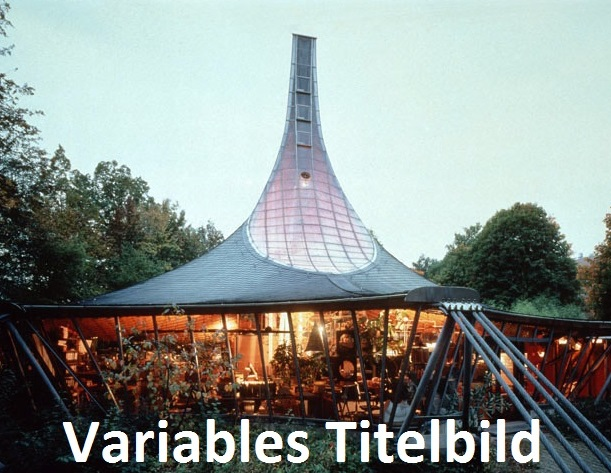
\includegraphics[width=1.0\textwidth]{Titelbild.jpg}
		\end{minipage}
	
	
		\vspace{10mm}
		
		\begin{minipage}[c]{4\baselineskip}
			\vspace{-1mm}
			
\includegraphics[height=3.5\baselineskip]{unistuttgart_logo_de.jpg}
		\end{minipage}
		\begin{minipage}[c]{90mm}
			\small \textsf{Universität Stuttgart} \\
    		\small \textsf{\Institut} \\
    		\small \textsf{\ProfEins} \\
    		\small \textsf{\ProfZwei} 
		\end{minipage}

	\end{minipage}
	\cleardoublepage
\end{titlepage}
%------------------------------------------------------------

\restoregeometry

\pagestyle{plain.scrheadings} % Leere Kopf- und Fußzeilen
\pagenumbering{Roman} % Römische Seitenzahlen verwenden
\addcontentsline{toc}{chapter}{Aufgabenstellung}

\includepdf[pages=-]{aufgabenstellung.pdf}  %->Optional
\chapter*{Eidesstattliche Erklärung}
\addcontentsline{toc}{chapter}{Eidesstattliche Erklärung}
\label{erklaerung}
Hiermit erkläre ich, dass ich die vorliegende Arbeit selbständig verfasst habe, dass ich keine anderen als die angegebenen Quellen benutzt und alle wörtlich oder sinngemäß aus anderen Werken übernommenen Aussagen als solche gekennzeichnet habe, dass die eingereichte Arbeit weder vollständig noch in wesentlichen Teilen Gegenstand eines anderen Prüfungsverfahrens gewesen ist, dass ich die Arbeit weder vollständig noch in Teilen bereits veröffentlicht habe und dass das elektronische Exemplar mit den anderen Exemplaren übereinstimmt. \\
\\[1.5cm]
Datum:	\hrulefill\enspace Unterschrift: \hrulefill
\\[3.5cm]
\chapter*{Vorwort}
\addcontentsline{toc}{chapter}{Vorwort}
\label{danksagungen}

\begin{description}
	\item[-] Diese Vorlage dient als grober Leitfaden zu Erstellung der Abschlussarbeit. Die Formatierung ist somit nicht zwingend umzusetzen.
	\item[-] Die Formatierung des Deckblattes sollte, soweit möglich, unverändert bleiben. 
	\item[-] Von der Gliederung der Arbeit kann abgewichen werden, solang dieses sinnig begründbar ist.
\end{description}
\vspace{10mm}
Um mit \LaTeX{} zu Arbeiten, kann z.B. die Kombination folgende Programme verwendet werden.
\begin{flalign*}
&\text{1) MiKTeX:} &&\text{\url{https://miktex.org/download}}&\\
&\text{2) TeXstudio:} &&\text{\url{https://www.texstudio.org/}}
\end{flalign*}
Alternativ besteht auch die Möglichkeit Online-Dienste zu benutzen, welche mögliche Schwierigkeiten bei der Einrichtung umgehen.

\subsection*{Empfohlene Einstellungen dieser Vorlage}
Für eine problemlose Kompilierung des \LaTeX-Dokumentes ist es notwendig, einige Einstellungen in den Editor zu übernehmen.
\begin{description}
	\item[-] Als Standard Bibliographieprogramm sollte Biber ausgewählt werden
	\item[-] Als Standardcompiler ist LuaLaTeX oder PdfLaTeX zu empfehlen
\end{description} %->Optional
\chapter*{Zusammenfassung}\addcontentsline{toc}{chapter}{Zusammenfassung}
\blindtext

\blindtext


\chapter*{Abstract}
\blindtext

\blindtext
\tableofcontents %Inhaltsverzeichnis
\cleardoubleoddpage %Beginn auf einer neuen Seite. Bei Doppelseiten rechts
\pagenumbering{arabic}	% Arabische Seitenzahlen verwenden
\chapter*{Bezeichnungen und Symbole}
\addcontentsline{toc}{chapter}{Bezeichnungen und Symbole}
\begin{longtable}{
		@{}
		>{\centering}p{0.15\linewidth}
		@{}
		>{\hspace*{0pt}}p{0.845\linewidth}
		@{}
	}
	\centering
	\small
	\tabularnewline
	\multicolumn{2}{@{}l}{\textsf{\textbf{Akronyme}}} \\
	APDL & Ansys Parametric Design Language \\
	DMS & Dehnungsmessstreifen \\
	FEM & Finite-Elemente-Methode \\
	
	\tabularnewline
	\multicolumn{2}{@{}l}{\textsf{\textbf{Lateinische Buchstaben}}} \\
	\textit{a} & Erster Eintrag \\
	\textit{b} & Zweiter Eintrag \\
	
	\tabularnewline
	\multicolumn{2}{@{}l}{\textsf{\textbf{Griechische Buchstaben}}} \\
	$\alpha$ & Kontinuierlicher Temperaturabminderungsfaktor \\
	$\varepsilon$ & Dehnung \\
	$\varepsilon_\mathrm{b}$ & Rechnerische Dehnung im Vierpunktbiegeversuch \\
	
	\tabularnewline
	\multicolumn{2}{@{}l}{\textsf{\textbf{Indizes}}} \\
	aktiv & Wert im aktiven Zustand \\
	min & Minimalwert \\
	
\end{longtable}
\cleardoubleoddpage %Beginn auf einer neuen Seite. Bei Doppelseiten rechts
\pagestyle{scrheadings}	% pagestyle für gesamtes Dokument aktivieren (Kopf- und Fußzeilen)


% ============= Kapitel =============
% durch Eigene Kapitel erstezen

\chapter{Grundlagen}
\label{sec:grundlagen}

\section{Zitation}
Nachfolgend Beispiele der Zitation in {\LaTeX} \cite{yang_application_2003}.
\blindtext
\cite{test}
\blindtext
\cite{kroll_computational_2016, yang_application_2003}


\section{Float Objekte}


\begin{description}
	\item[h:] an der Stelle, an der es in der Eingabedatei angegeben ist (here)
	\item[t:] am oberen Ende der aktuellen oder Folgeseite (top)
	\item[b:] am unteren Ende der aktuellen Seite (bottom)
	\item[p:] auf einer eigenen Seite für ein oder mehrere Gleitobjekte (page)
	\item[!:] Überschreiben Sie die internen Parameter, die LaTeX zur Bestimmung "guter"\\Gleitkommapositionen verwendet.
	\item[H:] Setzt den Float an genau die Stelle im LaTeX-Code. Erfordert das float-Paket.
\end{description}

\section{Einheiten}
Bei der Verwendung von Einheiten wird in der Regel bei Wissenschaftlichen Arbeiten ein schmales Leerzeichen verwendet.\\
1 m : Leerzeichen \\
1\,m : schmales Leerzeichen \\

\section{Gliederung: Beispiel Section}
\subsection{Gliederung: Beispiel Subsection}
\subsubsection{Gliederung: Beispiel Subsubsection}
Subsubsections werden, in dieser Vorlage, im Inhaltsverzeichnis aus Gründen der Übersichtlichkeit nicht abgebildet. % Zitation
\chapter{Einfügen von Quellcode}
\label{chap:code}

\section{Beispiel für einen Programmcode}


\if 1\mintedinstall
\subsection{Beispiel Minted}
	\begin{minted}[xleftmargin=20pt,linenos]{python}
	import numpy as np
	
	def incmatrix(genl1,genl2):
		m = len(genl1)
		n = len(genl2)
		M = None #to become the incidence matrix
		VT = np.zeros((n*m,1), int)  #dummy variable
	
		#compute the bitwise xor matrix
		M1 = bitxormatrix(genl1)
		M2 = np.triu(bitxormatrix(genl2),1) 
	
		for i in range(m-1):
			for j in range(i+1, m):
				[r,c] = np.where(M2 == M1[i,j])
				for k in range(len(r)):
					VT[(i)*n + r[k]] = 1;
					VT[(i)*n + c[k]] = 1;
					VT[(j)*n + r[k]] = 1;
					VT[(j)*n + c[k]] = 1;
					
					if M is None:
						M = np.copy(VT)
					else:
						M = np.concatenate((M, VT), 1)
					
					VT = np.zeros((n*m,1), int)
	
		return M
	\end{minted}
\fi




\subsection{Beispiel listings}
\begin{lstlisting}[language=Python]
import numpy as np

def incmatrix(genl1,genl2):
	m = len(genl1)
	n = len(genl2)
	M = None #to become the incidence matrix
	VT = np.zeros((n*m,1), int)  #dummy variable

	#compute the bitwise xor matrix
	M1 = bitxormatrix(genl1)
	M2 = np.triu(bitxormatrix(genl2),1) 
	
	for i in range(m-1):
		for j in range(i+1, m):
			[r,c] = np.where(M2 == M1[i,j])
			for k in range(len(r)):
				VT[(i)*n + r[k]] = 1;
				VT[(i)*n + c[k]] = 1;
				VT[(j)*n + r[k]] = 1;
				VT[(j)*n + c[k]] = 1;
	
				if M is None:
					M = np.copy(VT)
				else:
					M = np.concatenate((M, VT), 1)
				
				VT = np.zeros((n*m,1), int)
				
	return M
\end{lstlisting}

 % Programmcode
\chapter{Einfügen von Tabellen}
\label{chap:tabellen}

\section{Beispieltabelle}

\begin{table}[h]
	\caption{Beispieltabelle}
	\label{tab:Parameter}
	\centering
	\begin{tabularx}{\textwidth}{p{0.32\textwidth}p{0.32\textwidth}p{0.32\textwidth}}
																					\toprule
		Eins                       	     & Zwei    			& Drei 				\\ 	\midrule
		Vier                       	     & Fünf    			& Sechs				\\
		Sieben                           & Acht         	& Neun				\\ 	\bottomrule	
	\end{tabularx}
\end{table}

\begin{longtabu} to \textwidth {@{} X X[c] X[r] @{}}
	\caption{Tabelle auf Textbreite mit drei gleich großen Spalten}\label{tab:bsp1} \\
	\toprule
	Spalte 1 linksbündig & Spalte 2 zentriert & Spalte 3 rechtsbündig \\
	\midrule
1 , 2                           & 3 , 2                           & 1 , 3 \\
2 , 4                           & 6 , 4                           & 2 , 6 \\
3 , 6                           & 9 , 6                           & 3 , 9 \\
	\bottomrule
\end{longtabu}

\begin{longtabu} to 140mm {@{} X X[c] X[r] @{}}
	\caption{Tabelle auf Textbreite mit drei gleich großen Spalten}\label{tab:bsp2} \\
	\toprule
	Spalte 1 linksbündig & Spalte 2 zentriert & Spalte 3 rechtsbündig \\
	\midrule
1 , 2                           & 3 , 2                           & 1 , 3 \\
2 , 4                           & 6 , 4                           & 2 , 6 \\
3 , 6                           & 9 , 6                           & 3 , 9 \\
	\bottomrule
\end{longtabu}
%

\begin{longtabu} to \textwidth {@{} X[1,l] X[1,c] X[1,r] @{}}
	%----- Kopfzeile erste Tabelle ----- %
	\caption{Tabelle über mehrere Seiten}\label{tab:mehrere Seiten} \\
	\toprule
	Spalte 1 linksbündig & Spalte 2 zentriert & Spalte 3 rechtsbündig \\
	\midrule
	\endfirsthead
	%----- Kopfzeile zweite Tabelle ----- %	
	\caption*{\textbf{Fortsetzung:} \cref{tab:mehrere Seiten}} \\
	\toprule
	Spalte 1 linksbündig & Spalte 2 zentriert & Spalte 3 rechtsbündig \\
	\midrule
	\endhead
	%----- Tabellenende erste Tabelle ----- %	
	\bottomrule
	\endfoot
	%----- Tabellenende zweite Tabelle ----- %
	\bottomrule    
	\endlastfoot
	%----- Inhalt der Tabelle Tabelle ----- %	
1 , 2                           & 3 , 2                           & 1 , 3 \\
2 , 4                           & 6 , 4                           & 2 , 6 \\
3 , 6                           & 9 , 6                           & 3 , 9 \\
4 , 8                           & 12 , 8                           & 4 , 12 \\
5 , 10                           & 15 , 10                           & 5 , 15 \\
6 , 12                           & 18 , 12                           & 6 , 18 \\
7 , 14                           & 21 , 14                           & 7 , 21 \\
8 , 16                           & 24 , 16                           & 8 , 24 \\
9 , 18                           & 27 , 18                           & 9 , 27 \\
10 , 20                           & 30 , 20                           & 10 , 30 \\
11 , 22                           & 33 , 22                           & 11 , 33 \\
12 , 24                           & 36 , 24                           & 12 , 36 \\
13 , 26                           & 39 , 26                           & 13 , 39 \\
14 , 28                           & 42 , 28                           & 14 , 42 \\
15 , 30                           & 45 , 30                           & 15 , 45 \\
16 , 32                           & 48 , 32                           & 16 , 48 \\
17 , 34                           & 51 , 34                           & 17 , 51 \\
18 , 36                           & 54 , 36                           & 18 , 54 \\
19 , 38                           & 57 , 38                           & 19 , 57 \\
\end{longtabu} % Tabellen
\chapter{Mathematische Beispiele}
\label{sec:math}


\section{Gleichungen}

\begin{align}
\sin A \cos B &= \frac{1}{2}\left[ \sin(A-B)+\sin(A+B) \right] \\
\sin A \sin B &= \frac{1}{2}\left[ \sin(A-B)-\cos(A+B) \right] \\
\cos A \cos B &= \frac{1}{2}\left[ \cos(A-B)+\cos(A+B) \right] 
\end{align}

\begin{align*}
\sin A \cos B &= \frac{1}{2}\left[ \sin(A-B)+\sin(A+B) \right] \\
\sin A \sin B &= \frac{1}{2}\left[ \sin(A-B)-\cos(A+B) \right] \\
\cos A \cos B &= \frac{1}{2}\left[ \cos(A-B)+\cos(A+B) \right] 
\end{align*}

\[
\int_a^bu\frac{d^2v}{dx^2}\,dx
=\left.u\frac{dv}{dx}\right|_a^b
-\int_a^b\frac{du}{dx}\frac{dv}{dx}\,dx.
\]



\section{Arrays}

\[
\begin{bmatrix}
1 & x & 0 \\
0 & 1 & -1
\end{bmatrix}\begin{bmatrix}
1  \\
y  \\
1
\end{bmatrix}
=\begin{bmatrix}
1+xy  \\
y-1
\end{bmatrix}.
\]


\[
|x|=\begin{cases}
x, & \text{if }x\geq 0\,,  \\
-x, & \text{if }x< 0\,.
\end{cases}
\]


\[
\begin{matrix}
-2 & 1 & 0 & 0 & \cdots & 0  \\
1 & -2 & 1 & 0 & \cdots & 0  \\
0 & 1 & -2 & 1 & \cdots & 0  \\
0 & 0 & 1 & -2 & \ddots & \vdots \\
\vdots & \vdots & \vdots & \ddots & \ddots & 1  \\
0 & 0 & 0 & \cdots & 1 & -2
\end{matrix}
\]





 % Formeln
\chapter{tikz - Grafiken}
\label{sec:tikz}

\section{Beispielkapitel tikz - Grafiken}
\label{sec:beispiel}

\subsection{Darstellung von Funktionen}

\begin{figure}[htb]
\centering
\begin{align*}
f(x)=\tanh(x)
\end{align*}
\begin{tikzpicture}
\begin{axis}
[
width=200pt,
height=200pt,
axis x line=middle, xmin=-4, xmax=4, xtick={-3,...,3}, xlabel=$x$,
axis y line=middle, ymin=-1.5, ymax=1.5, ytick={-1,...,1}, ylabel=$f(x)$,
scale only axis=true,
samples=101
]
\addplot[uniSdarkblue, mark=none, very thick]{tanh(x)};
%		\legend{$\tanh(x)$}
\end{axis}
\end{tikzpicture}
\caption[Tangens hyperbolicus Aktivierungsfunktion]{Tangens hyperbolicus}
\label{fig:AktivTan}
\end{figure}

\newpage
\subsection{for-Schleifen bei der Grafikerzeugung}

\begin{figure}[htb]
	\centering
	\begin{tikzpicture}[]
	\tikzstyle{netnode}=[circle, inner sep=0pt, text width=22pt, align=center, line width=1.0pt]
	\tikzstyle{inputnode}=[netnode, fill=uniSlightgrey,draw=black]
	\tikzstyle{hiddennode}=[netnode, fill=uniSlightgrey,draw=black]
	\tikzstyle{outputnode}=[netnode, fill=uniSlightgrey,draw=black]
	\tikzstyle{signal}=[arrows={-latex},draw=uniSblack,line width=1pt,rounded corners=4pt]
	
	\def\nodedist{35pt}
	\def\layerdist{80pt}
	\def\pindist{20pt}
	
	\tikzstyle{every pin edge}=[signal]
	\tikzstyle{annot} = [text width=6em, text centered]
	
	\foreach \y in {1,...,3}
	\node[inputnode, pin={[pin edge={latex-}, pin distance=\pindist]left:Eingabe \y}] 
	(I\y) at (0,-\y*\nodedist) {$i_\y$};  
	
	\foreach \y in {1,...,4}
	\node[hiddennode] 
	(H1\y) at ($(\layerdist,-\y*\nodedist) +(0, 0.5*\nodedist)$) {$h_\y^1$};
	
	\foreach \y in {1,...,4}
	\node[hiddennode] 
	(H2\y) at ($(2*\layerdist,-\y*\nodedist) +(0, 0.5*\nodedist)$) {$h_\y^2$};
	
	\foreach \y in {1,...,2}
	\node[outputnode, pin={[pin edge={-latex}, pin distance=\pindist]right:Ausgabe \y}]
	(O\y) at ($(H21) + (\layerdist, -\y*\nodedist)$) {$o_\y$};
	
	\foreach \dest in {1,...,4}
	\foreach \source in {1,...,3}
	\draw[signal] (I\source) -- (H1\dest);
	
	\foreach \dest in {1,...,4}
	\foreach \source in {1,...,4}
	\draw[signal] (H1\source) -- (H2\dest);
	
	\foreach \dest in {1,...,2}
	\foreach \source in {1,...,4}
	\draw[signal] (H2\source) edge (O\dest);
	
	\node[annot, above=4pt of H11] (hl) {verborgene Schicht 1};
	\node[annot, above=4pt of H21] (hl) {verborgene Schicht 2};
	\node[annot] at (I1 |- hl) {Eingabe\-schicht};
	\node[annot] at (O1 |- hl) {Ausgabe\-schicht};
	\end{tikzpicture}
	\caption[Schematischer Aufbau eines künstlichen neuronalen Netzes] %hier kann ein alternativer/ verkürzter Text für das Abbildungsverzeichnis angegeben werden
	{Schematischer Aufbau eines künstlichen neuronalen Netzes \cite[Abb. nach][]{Frochte.2019}} %Bildunteschrift
	\label{fig:DNN}
\end{figure}


\subsection{Einbeziehung von Daten aus CSV-Datei}

\setlength{\figureheight}{5cm}
\setlength{\figurewidth}{\textwidth}
\begin{figure}[htbp]
	\centering
	\begin{tikzpicture}
		\begin{axis}[
			width=\figurewidth,
			height=\figureheight,
			date coordinates in = x,
			xmin=2018-01-01 00:00,
			xmax=2018-01-08 00:00,
			minor x tick num=1,
			xtick={2018-01-01 12:00, 2018-01-02 12:00, 2018-01-03 12:00, 2018-01-04 12:00, 2018-01-05 12:00, 2018-01-06 12:00, 2018-01-07 12:00},
			set layers,cell picture=true,
			xticklabel={\day.\month},
			xlabel={2018},
			ymin=-0.1, ymax=1.1, ytick={0,0.5,1},
			no marks,
			scaled y ticks = false,
			ylabel={[\nicefrac{\%}{100}]}
			,]
			\addplot+[color=black ] table[x=Zeit, y=Shadestep, col sep=comma, skip first n=0] {./02_data/Example.csv};
			\legend{Shadestep};
		\end{axis}
	\end{tikzpicture}
	\caption[Photometrische Regelung der adaptiven Verglasung im Juli 2018, nach 500 Episoden]{Photometrische Regelung der adaptiven Verglasung nach 500 Episoden, für den Zeitraum vom 01. bis 07. Juli 2018} \label{fig:AVPhJun500}	
\end{figure}

\newpage
\subsection{Einbeziehung von Daten aus CSV-Datei und Gruppierung von Grafiken}

\begin{figure}[htb]
	\setlength{\figureheight}{5cm}
	\setlength{\figurewidth}{\textwidth}
	\centering
	\begin{tikzpicture}
		\begin{groupplot}[
			width=\figurewidth,
			height=\figureheight,
			date coordinates in = x,
			xmin=2018-01-01 00:00,
			xmax=2018-01-08 00:00,
			minor x tick num=1,
			xtick={2018-01-01 12:00, 2018-01-02 12:00, 2018-01-03 12:00, 2018-01-04 12:00, 2018-01-05 12:00, 2018-01-06 12:00, 2018-01-07 12:00},
			set layers,cell picture=true,
			xticklabel={\day.\month},
			xlabel={2018},
			no marks,
			scaled y ticks = false,
			group style = {group size = 1 by 7,
				horizontal sep =1cm,
				vertical sep = 0cm,},]
			
			\nextgroupplot[xlabel={},xticklabels={},ylabel={[°C]}]
			\addplot[color=black ] table[x=Zeit, y=T01, col sep=comma, skip first n=0] {./02_data/Example.csv};
			\legend{T01};
			
			\nextgroupplot[xlabel={},xticklabels={},ylabel={[klx]}]
			\addplot[color=black ] table[x=Zeit, y expr=\thisrow{B01}/1000, col sep=comma, skip first n=0] {./02_data/Example.csv};
			\legend{B01};
			
			\nextgroupplot[ylabel={[kW]}, ymin=-0.02, ymax=0.32, ytick={0,0.1,0.2,0.3},]
			\addplot+[color=black , name path=A] table[x=Zeit, y expr=\thisrow{QBeleuchtung}+\thisrow{QHeizung}+\thisrow{QKuehlung}, col sep=comma, skip first n=0] {./02_data/Example.csv};
			\addplot+[draw=none,name path=B, mark=none] table[x=Zeit, y expr=0, col sep=comma, skip first n=0] {./02_data/Example.csv}; 
			\addplot+[gray, fill opacity=0.1] fill between[of=A and B];
			\legend{Q\textsubscript{HEAT}+Q\textsubscript{COOL}+Q\textsubscript{LIGHT}};

		\end{groupplot}
	\end{tikzpicture}
	\caption[Kombinierte Regelung im Januar 2018, nach 500 Episoden]{Kombinierte Regelung nach 500 Episoden, für den Zeitraum vom 01. bis 07. Januar 2018} \label{fig:KomJan18}	
\end{figure}


\section{Beispielkapitel Standard Grafik}
\label{sec:graf}

\subsection{Einfaches Bild}

\begin{figure}[H]
  \centering  
  	
\includegraphics[scale=0.5]{ILEK-logo.jpg}
  \caption{ILEK Logo}
  \label{fig:starwars}
\end{figure}

\subsection{Gruppierung von Bildern}

\begin{figure}[H]
	\centering
	\begin{subfigure}[b]{0.3\textwidth}
		\centering
		
\includegraphics[width=\textwidth]{ILEK-logo.jpg}
		\caption{$y=x$}
		\label{fig:a}
	\end{subfigure}
%	\hfill
\hspace{1cm}
	\begin{subfigure}[b]{0.3\textwidth}
		\centering
		
\includegraphics[width=\textwidth]{ILEK-logo.jpg}
		\caption{$y=3sinx$}
		\label{fig:b}
	\end{subfigure}
	\\ 
	\begin{subfigure}[b]{0.3\textwidth}
		\centering
		
\includegraphics[width=\textwidth]{ILEK-logo.jpg}
		\caption{$y=3sinx$}
		\label{fig:c}
	\end{subfigure}
%	\hfill
\hspace{1cm}
	\begin{subfigure}[b]{0.3\textwidth}
		\centering
		
\includegraphics[width=\textwidth]{ILEK-logo.jpg}
		\caption{$y=5/x$}
		\label{fig:five over x}
	\end{subfigure}
	\caption{Vier Bilder}
	\label{fig:d}
\end{figure}

\subsection{Bilder und Tabellen im Fließtext}

\begin{wraptable}[]{o}[0cm]{9cm}
	\begin{center}
		\begin{tabular}{|l|l|l|}
			\hline
			r & R & right side of the text\\
			l & L & left side of the text\\
			i & I & inside edge–near the binding\\
			& &  (in a twoside document)\\
			o & O & outside edge–far from the binding\\
			\hline
		\end{tabular}
	\end{center}
	\caption{The uppercase version allows the figure to float. The lowercase version means exactly here.}%\citep{cite}
\end{wraptable}

\blindtext[2]

%\begin{wrapfigure}[Zeile]{Position}[Randüberhang]{Breite}
\begin{wrapfigure}[]{o}[0cm]{6.5cm}
	\begin{center}
	
\includegraphics[width=5cm,angle=0]{ILEK-logo.jpg}
	\caption{Bildbezeichnung}
	\label{fig:bild}
	\end{center}
\end{wrapfigure}

\blindtext[2] % Grafiken
\chapter{Exemplarischer Anhang}
\label{chap:tab}

\section{Beispieltabelle}

\begin{table}[h]
	\caption{Beispieltabelle}
	\label{tab:par}
	\centering
	\begin{tabularx}{\textwidth}{p{0.32\textwidth}p{0.32\textwidth}p{0.32\textwidth}}
																					\toprule
		Eins                       	     & Zwei    			& Drei 				\\ 	\midrule
		Vier                       	     & Fünf    			& Sechs				\\
		Sieben                           & Acht         	& Neun				\\ 	\bottomrule	
	\end{tabularx}
\end{table}

\begin{longtabu} to \textwidth {@{} X X[c] X[r] @{}}
	\caption{Tabelle auf Textbreite mit drei gleich großen Spalten} \\
	\toprule
	Spalte 1 linksbündig & Spalte 2 zentriert & Spalte 3 rechtsbündig \\
	\midrule
1 , 2                           & 3 , 2                           & 1 , 3 \\
2 , 4                           & 6 , 4                           & 2 , 6 \\
3 , 6                           & 9 , 6                           & 3 , 9 \\
	\bottomrule
\end{longtabu}

\begin{longtabu} to 140mm {@{} X X[c] X[r] @{}}
	\caption{Tabelle auf Textbreite mit drei gleich großen Spalten} \\
	\toprule
	Spalte 1 linksbündig & Spalte 2 zentriert & Spalte 3 rechtsbündig \\
	\midrule
1 , 2                           & 3 , 2                           & 1 , 3 \\
2 , 4                           & 6 , 4                           & 2 , 6 \\
3 , 6                           & 9 , 6                           & 3 , 9 \\
	\bottomrule
\end{longtabu}

\begin{longtabu} to \textwidth {@{} X[1,l] X[1,c] X[1,r] @{}}
	%----- Kopfzeile erste Tabelle ----- %
	\caption{Tabelle über mehrere Seiten}\label{tab:mehrere Seiten Anhang} \\
	\toprule
	Spalte 1 linksbündig & Spalte 2 zentriert & Spalte 3 rechtsbündig \\
	\midrule
	\endfirsthead
	%----- Kopfzeile zweite Tabelle ----- %	
	\caption*{\textbf{Fortsetzung:} \Cref{tab:mehrere Seiten Anhang}} \\
	\toprule
	Spalte 1 linksbündig & Spalte 2 zentriert & Spalte 3 rechtsbündig \\
	\midrule
	\endhead
	%----- Tabellenende erste Tabelle ----- %	
	\bottomrule
	\endfoot
	%----- Tabellenende zweite Tabelle ----- %
	\bottomrule    
	\endlastfoot
	%----- Inhalt der Tabelle Tabelle ----- %	
	1 , 2                           & 3 , 2                           & 1 , 3 \\
	2 , 4                           & 6 , 4                           & 2 , 6 \\
	3 , 6                           & 9 , 6                           & 3 , 9 \\
	4 , 8                           & 12 , 8                           & 4 , 12 \\
	5 , 10                           & 15 , 10                           & 5 , 15 \\
	6 , 12                           & 18 , 12                           & 6 , 18 \\
	7 , 14                           & 21 , 14                           & 7 , 21 \\
	8 , 16                           & 24 , 16                           & 8 , 24 \\
	9 , 18                           & 27 , 18                           & 9 , 27 \\
	10 , 20                           & 30 , 20                           & 10 , 30 \\
	11 , 22                           & 33 , 22                           & 11 , 33 \\
	12 , 24                           & 36 , 24                           & 12 , 36 \\
	13 , 26                           & 39 , 26                           & 13 , 39 \\
	14 , 28                           & 42 , 28                           & 14 , 42 \\
	15 , 30                           & 45 , 30                           & 15 , 45 \\
	16 , 32                           & 48 , 32                           & 16 , 48 \\
	17 , 34                           & 51 , 34                           & 17 , 51 \\
	18 , 36                           & 54 , 36                           & 18 , 54 \\
	19 , 38                           & 57 , 38                           & 19 , 57 \\
\end{longtabu}
 % Anhang

\ifluatex
\chapter{Programmierungen}\label{chap:programming}
\section{{\TeX} if/ else}\label{sec:tex}
Grundlegender Aufbau:\\
\begin{lstlisting}[language=TeX]
\if <token-1><token-2> <tex-code-1> [\else <tex-code-2>] \fi
\end{lstlisting}
Bsp1:\\
\begin{lstlisting}[language=TeX]
\ifx\mycmd\undefined
	undefed
\else
	\if\mycmd1
		defed, 1
	\else
		defed
	\fi
\fi
\end{lstlisting}

\ifx\mycmd\undefined
	undefed
\else
	\if\mycmd1
		defed, 1
	\else
		defed
	\fi
\fi
\\Bsp2:\\
\begin{lstlisting}[language=TeX]
\def\mycmd{1}

\ifx\mycmd\undefined
	undefed
\else
	\if\mycmd1
		defed, 1
	\else
		defed
	\fi
\fi
	
\end{lstlisting}

\def\mycmd{1}

\ifx\mycmd\undefined
	undefed
\else
	\if\mycmd1
		defed, 1
	\else
		defed
	\fi
\fi
\\Bsp3:\\
\begin{lstlisting}[language=TeX]
\def\mycmd{0}

\ifx\mycmd\undefined
	undefed
\else
	\if\mycmd1
		defed, 1
	\else
		defed
	\fi
\fi
\end{lstlisting}


\def\mycmd{0}

\ifx\mycmd\undefined
	undefed
\else
	\if\mycmd1
		defed, 1
	\else
		defed
	\fi
\fi


\section{forPGF}\label{sec:pgf}

\section{Lua}\label{sec:lua}
\begin{lstlisting}[language={[5.0]Lua}]
\count75=1564 % Data existing in the "TeX World"
\directlua{
local x=\number\count75 \space % Transfer TeX data to the "Lua World"
tex.print("x= "..x)
local y = (2*x-65)/5
tex.print(" and y = "..y)
}
\end{lstlisting}

%\count75=1564 % Data existing in the "TeX World"
%\directlua{
%local x=\number\count75 \space % Transfer TeX data to the "Lua World"
%tex.print("x= "..x)
%local y = (2*x-65)/5
%tex.print(" and y = "..y)
%}

Die Kreiszahl $\pi$ hat den Wert \directlua{tex.print(math.pi)}.

\def\aa{tex}
\def\bb{.}
\def\cc{print}
\def\dd{("Hello wie gehts")}
\directlua{\aa\bb\cc\dd}

\directlua{
	tex.print(math.random())
	tex.print(math.random())
}

 % Programmierung
\fi

% ============= Anhang =============

%\appendix
%\begin{appendices}
%	\chapter{Exemplarischer Anhang}
\label{chap:tab}

\section{Beispieltabelle}

\begin{table}[h]
	\caption{Beispieltabelle}
	\label{tab:par}
	\centering
	\begin{tabularx}{\textwidth}{p{0.32\textwidth}p{0.32\textwidth}p{0.32\textwidth}}
																					\toprule
		Eins                       	     & Zwei    			& Drei 				\\ 	\midrule
		Vier                       	     & Fünf    			& Sechs				\\
		Sieben                           & Acht         	& Neun				\\ 	\bottomrule	
	\end{tabularx}
\end{table}

\begin{longtabu} to \textwidth {@{} X X[c] X[r] @{}}
	\caption{Tabelle auf Textbreite mit drei gleich großen Spalten} \\
	\toprule
	Spalte 1 linksbündig & Spalte 2 zentriert & Spalte 3 rechtsbündig \\
	\midrule
1 , 2                           & 3 , 2                           & 1 , 3 \\
2 , 4                           & 6 , 4                           & 2 , 6 \\
3 , 6                           & 9 , 6                           & 3 , 9 \\
	\bottomrule
\end{longtabu}

\begin{longtabu} to 140mm {@{} X X[c] X[r] @{}}
	\caption{Tabelle auf Textbreite mit drei gleich großen Spalten} \\
	\toprule
	Spalte 1 linksbündig & Spalte 2 zentriert & Spalte 3 rechtsbündig \\
	\midrule
1 , 2                           & 3 , 2                           & 1 , 3 \\
2 , 4                           & 6 , 4                           & 2 , 6 \\
3 , 6                           & 9 , 6                           & 3 , 9 \\
	\bottomrule
\end{longtabu}

\begin{longtabu} to \textwidth {@{} X[1,l] X[1,c] X[1,r] @{}}
	%----- Kopfzeile erste Tabelle ----- %
	\caption{Tabelle über mehrere Seiten}\label{tab:mehrere Seiten Anhang} \\
	\toprule
	Spalte 1 linksbündig & Spalte 2 zentriert & Spalte 3 rechtsbündig \\
	\midrule
	\endfirsthead
	%----- Kopfzeile zweite Tabelle ----- %	
	\caption*{\textbf{Fortsetzung:} \Cref{tab:mehrere Seiten Anhang}} \\
	\toprule
	Spalte 1 linksbündig & Spalte 2 zentriert & Spalte 3 rechtsbündig \\
	\midrule
	\endhead
	%----- Tabellenende erste Tabelle ----- %	
	\bottomrule
	\endfoot
	%----- Tabellenende zweite Tabelle ----- %
	\bottomrule    
	\endlastfoot
	%----- Inhalt der Tabelle Tabelle ----- %	
	1 , 2                           & 3 , 2                           & 1 , 3 \\
	2 , 4                           & 6 , 4                           & 2 , 6 \\
	3 , 6                           & 9 , 6                           & 3 , 9 \\
	4 , 8                           & 12 , 8                           & 4 , 12 \\
	5 , 10                           & 15 , 10                           & 5 , 15 \\
	6 , 12                           & 18 , 12                           & 6 , 18 \\
	7 , 14                           & 21 , 14                           & 7 , 21 \\
	8 , 16                           & 24 , 16                           & 8 , 24 \\
	9 , 18                           & 27 , 18                           & 9 , 27 \\
	10 , 20                           & 30 , 20                           & 10 , 30 \\
	11 , 22                           & 33 , 22                           & 11 , 33 \\
	12 , 24                           & 36 , 24                           & 12 , 36 \\
	13 , 26                           & 39 , 26                           & 13 , 39 \\
	14 , 28                           & 42 , 28                           & 14 , 42 \\
	15 , 30                           & 45 , 30                           & 15 , 45 \\
	16 , 32                           & 48 , 32                           & 16 , 48 \\
	17 , 34                           & 51 , 34                           & 17 , 51 \\
	18 , 36                           & 54 , 36                           & 18 , 54 \\
	19 , 38                           & 57 , 38                           & 19 , 57 \\
\end{longtabu}

%\end{appendices}


% ============= Verzeichnise =============

\printbibliography[title=Literaturverzeichnis] %Literaturverzeichnis
\addcontentsline{toc}{chapter}{Literaturverzeichnis}

\listoffigures %Verzeichnis aller Bilder
\addcontentsline{toc}{chapter}{Abbildungsverzeichnis}

\listoftables %Verzeichnis aller Tabellen
\addcontentsline{toc}{chapter}{Tabellenverzeichnis}


% ============= Dokumentende =============

\end{document}
